\chapter{Studio di funzione completo}
Proponiamo qui una traccia per studiare una funzione al fine di produrre un grafico probabile. Non è necessario né svolgere tutti i punti né svolgerli in ordine. Si consiglia di iniziare da subito a tracciare il grafico e di aggiornarlo man mano in mado di verificare progressivamente tutte le parti dello studio di funzione. Di seguito si riportano alcuni esempi.
\section{Traccia per lo studio di funzione completo}
    \subsection{Classificazione}
    \begin{tabular}{|c|c|c|c|}
        \hline
        \multirow{2}{4em}{Funzione} & algebrica\ & razionale & intera\\ \cline{2-4}
         & trascendente & irrazionale & fratta \\ \hline
    \end{tabular}
    \subsection{Dominio}
    \begin{itemize}
        \item Polinomiale : $\R$
        \item Fratte: denominatore $\neq 0$
        \item Irrazionali pari: radicando$\geq0$
        \item Irrazionali dispari: $\R$
        \item Logaritmi: argomento$>0$
        \item Esponenziali: $\R$
        \item Seno, coseno, arcotangente, arcocotangente: $\R$
        \item Tangente: $\R \setminus \{\frac{\pi}{2}+k\pi\}\text{, con } k\in\Z$
        \item Cotangente: $\R \setminus \{k\pi\}\text{, con } k\in\Z$
        \item Arcoseno, arcocoseno: $[-1;1]$
    \end{itemize}
    \subsection{Simmetrie}
    \textbf{CN:} $\forall x \in D, -x \in D$
    \begin{itemize}
        \item pari se $f(-x)=f(x)$
        \item dispari se $f(-x)=-f(x)$
    \end{itemize}
    \subsection{Intersezioni con gli assi cartesiani}
    \[f(x) \cap \text{asse~}x : \left\{\begin{array}{l}
         y=f(x)  \\
         y=0 
    \end{array}\right.~~~~~~~~ 
    f(x) \cap \text{asse~}y : \left\{\begin{array}{l}
         y=f(x)  \\
         x=0 
    \end{array}\right.\] 
    \subsection{Studio del segno}
    Risolvere la disequazione $f(x)>0$
    \subsection{Limiti, asintoti e discontinuità}
    \begin{tabular}{|m{0.3\textwidth}|m{0.6\textwidth}|}
        \hline
        Asintoto verticale&  \[\lim_{x\rightarrow x_0} f(x) = \infty\] \\\hline
        Asintoto orizzontale & \[\lim_{x\rightarrow \infty} f(x) = l\]\\ \hline
        Asintoto obliquo & \[\textnormal{CN: }\lim_{x\rightarrow\infty}f(x) = \infty\]
        \[m=\lim_{x\rightarrow\infty}\frac{f(x)}{x}\]
        \[q=\lim_{x\rightarrow\infty}f(x)-mx\] \\ \hline
    \end{tabular}\\
    \\
    \textbf{NB.:} Una funzione può avere anche infiniti asintoti verticali, ma al massimo due tra asintoti orizzontali e asintoti obliqui (uno destro e uno sinistro).\\    \begin{tabular}{|m{0.3\textwidth}|m{0.6\textwidth}|}
        \hline
        Prima specie &  \[\lim_{x\rightarrow x_0^-}f(x)=l_1~~~~\lim_{x\rightarrow x_0^+}f(x)=l_2\] \[l_1\neq l_2~~~~salto=|l_1-l_2|\]\\ \hline
        Seconda specie &  \[\lim_{x\rightarrow x_0^\pm}f(x)=\infty ~~~~\lor~~~~ \lim_{x\rightarrow x_0^\pm}f(x)=\nexists\] \\\hline
        Terza specie & \[\lim_{x\rightarrow x_0^-}f(x)=\lim_{x\rightarrow x_0^+}f(x)=l\]\[f(x_0)\neq l ~~~~ \lor ~~~~ f(x_0)=\nexists\]\\ \hline
    \end{tabular}
    \subsection{Derivata prima}
    Le soluzioni dell'equazione \[f'(x) = 0\] identificano la presenza di \begin{itemize}
        \item massimi relativi
        \item minimi relativi
        \item flessi a tangente orizzontale
    \end{itemize}
    Per distinguerli è necessario studiare il segno della derivata:
    \begin{figure}[ht]
        \centering
        \begin{subfigure}{0.24\textwidth}
            \centering
            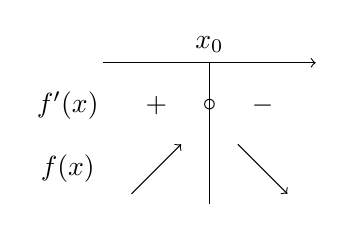
\begin{tikzpicture}[scale=0.9]
                \draw[->](0,0)--(3,0);
                \draw(1.5,0) node[above]{$x_0$}--(1.5,-2);
                \node at (-0.50, -0.60){$f'(x)$};
                \node at (-0.50, -1.50){$f(x)$};
                \node at (0.75,-0.60) {$+$};
                \node at (2.25,-0.60) {$-$};
                \node at (1.5, -0.60) {$\circ$};
                \draw[->] (0.4,-1.85)--(1.1,-1.15); %+ sx
                \draw[->] (1.9,-1.15)--(2.6,-1.85); %- dx
            \end{tikzpicture}
            \caption{Massimo relativo}
        \end{subfigure}
        \begin{subfigure}{0.24\textwidth}
            \centering
            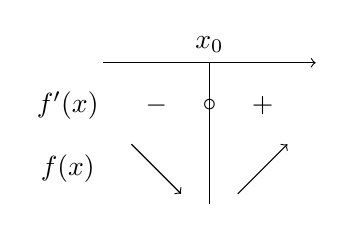
\begin{tikzpicture}[scale=0.9]
                \draw[->](0,0)--(3,0);
                \draw(1.5,0) node[above]{$x_0$}--(1.5,-2);
                \node at (-0.50, -0.60){$f'(x)$};
                \node at (-0.50, -1.50){$f(x)$};
                \node at (0.75,-0.60) {$-$};
                \node at (2.25,-0.60) {$+$};
                \node at (1.5, -0.60) {$\circ$};
                \draw[->] (0.4,-1.15)--(1.1,-1.85); %- sx
                \draw[->] (1.9,-1.85)--(2.6,-1.15); %+ dx
            \end{tikzpicture}
            \caption{Minimo relativo}
        \end{subfigure}
        \begin{subfigure}{0.24\textwidth}
            \centering
            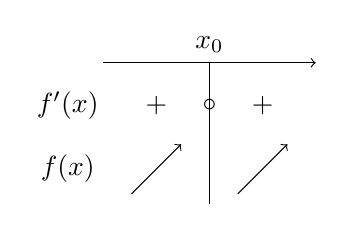
\begin{tikzpicture}[scale=0.9]
                \draw[->](0,0)--(3,0);
                \draw(1.5,0) node[above]{$x_0$}--(1.5,-2);
                \node at (-0.50, -0.60){$f'(x)$};
                \node at (-0.50, -1.50){$f(x)$};
                \node at (0.75,-0.60) {$+$};
                \node at (2.25,-0.60) {$+$};
                \node at (1.5, -0.60) {$\circ$};
                %\draw[->] (0.4,-1.15)--(1.1,-1.85); %- sx
                \draw[->] (0.4,-1.85)--(1.1,-1.15); %+ sx
                %\draw[->] (1.9,-1.15)--(2.6,-1.85); %- dx
                \draw[->] (1.9,-1.85)--(2.6,-1.15); %+ dx
            \end{tikzpicture}
            \caption{Flesso ascendente}
        \end{subfigure}
        \begin{subfigure}{0.24\textwidth}
            \centering
            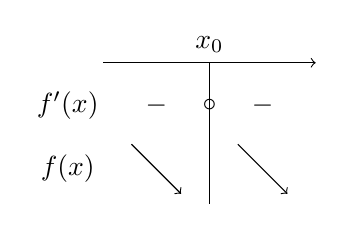
\begin{tikzpicture}[scale=0.9]
                \draw[->](0,0)--(3,0);
                \draw(1.5,0) node[above]{$x_0$}--(1.5,-2);
                \node at (-0.50, -0.60){$f'(x)$};
                \node at (-0.50, -1.50){$f(x)$};
                \node at (0.75,-0.60) {$-$};
                \node at (2.25,-0.60) {$-$};
                \node at (1.5, -0.60) {$\circ$};
                \draw[->] (0.4,-1.15)--(1.1,-1.85); %- sx
                \draw[->] (1.9,-1.15)--(2.6,-1.85); %- dx
            \end{tikzpicture}
            \caption{Flesso discendente}
        \end{subfigure}
        \caption{}
    \end{figure}
    Lo studio della derivata prima fornisce anche informazioni circa la monotonia della funzione.
    \subsection{Derivata seconda}
    Le soluzioni dell'equazione \[f''(x)=0\] permettono di identificare i punti di flesso. A differenza della derivata prima permette di ottenere informazioni circa la presenza di flessi a tangente obliqua, per cui è necessario escludere tutte le soluzioni già analizzate in precedenza. 
    La derivata seconda fornisce inoltre informazioni circa la concavità della funzione: verso l'alto quando la derivata seconda è positiva e verso il basso quando la derivata seconda è negativa. La funzione inverte la propria concavità in corrispondenza dei punti di flesso.
    \subsection{Estremi globali}
    In conclusione è opportuno elencare i punti di estremo globali, da ricercarsi tra gli estremi del dominio, i punti stazionari e i punti di non derivabilità.

\section{Esempi}
    \begin{ex}[Studiare la funzione $ y=\frac{x^2}{x-1}$.]
        \begin{enumerate}
            \item \textbf{Classificazione:} funzione algebrica razionale fratta;
            \item \textbf{Dominio:} $\dom f=\;]-\infty;1[\ \cup \ ]1;+\infty[$ 
            \item \textbf{Simmetrie:} il dominio non è simmetrico, per cui la condizione necessaria non è rispettata, di conseguenza la funzione non è né pari né dispari.
            \item \textbf{Intersezioni con gli assi:} è consigliabile partire dalle intersezioni con l'asse $x$, perchè potremmo trovare anche l'unica intersezione con l'asse $y$ nel caso la funzione passi per l'origine.
            \[f(x)=0\ \ \Harr \ \ x^2=0\ \ \Harr \ \ x=0.\]
            La funzione passa appunto per l'origine $O(0,0)$, quindi non ci serve calcolare anche l'intersezione con l'asse $y$.
            \item \textbf{Segno:} $f(x)>0$
            \begin{center}
                \begin{tikzpicture}
                    \node at (1,0.4) [anchor=west]{$N: x^2>0$};
                    \node at (1,-0.4)[anchor=west]{$D: (x-1)>0$};
                    \node at (1,-1.2)[anchor=west]{$\dom f: x\neq 1$};
                    \node at (5,0.4)[anchor=west]{$x\neq 0$};
                    \node at (5,-0.4)[anchor=west]{$x>1$};
                    \draw[->] (7.5,1)--(11.5,1);
                    \draw (8.75,1)node [above]{$0$}--(8.75,-2);
                    \draw (10.25,1) node [above]{$1$}--(10.25,-2);
                    \draw[color=red, dashed] (7.5, -0.4)--(10.25,-0.4) node {$\circ$};
                    %\draw[color=red] (8.75, 0.4)--(10.25,0.4) node {$\circ$};
                    \node [color=red] at (8.75,0.4){$\circ$};
                    \draw [color=red] (10.25, -0.4)--(11.5,-0.4);
                    \draw [color=red] (7.5, 0.4)--(11.5,0.4);
                    \draw [color=red] (7.5, -1.2)--(11.5,-1.2);
                    \node [color=red] at (10.25,-1.2){$\nexists$};
                    \node [color=red]at (8.125,-1.8){$-$};
                    \node [color=red]at (9.5,-1.8){$-$};
                    \node [color=red]at (11,-1.8){$+$};
                \end{tikzpicture}
            \end{center}
            \item \textbf{Limiti, asintoti e discontinuità:} Dobbiamo calcolare i limiti agli estremi del dominio:
            \[\lim_{x\to-\infty}\frac{\boxed{x^{\cancel{2}}}}{\cancel{\boxed{x}}-1}=\left[ \frac{\infty}{\infty} \right]\overset{FI}{=}-\infty \qquad \qquad \lim_{x\to+\infty}\frac{\boxed{x^{\cancel{2}}}}{\cancel{\boxed{x}}-1}=\left[ \frac{\infty}{\infty} \right]\overset{FI}{=}+\infty\]
            È verificata la condizione necessaria per la ricerca dell'asintoto obliquo, per cui procediamo con la ricerca dello stesso:
            \[m=\lim_{x\to\infty}\frac{{x^{{2}}}}{x({{x}}-1)}=\left[ \frac{\infty}{\infty} \right]\overset{FI}{=}\lim_{x\to\infty}\frac{x^2}{x^2-1}=1\]
            \[q=\lim_{x\to \infty}\left(\frac{x^2}{x-1}-x\right)=\lim_{x\to\infty}\frac{x^2-x^2+x}{x-1}=\left[ \frac{\infty}{\infty} \right]\overset{FI}{=}1.\]
            Per cui la funzione ha un asintoto obliquo (destro e sinistro) alla retta $y=x+1$
            \[\lim_{x\to1^-}\frac{x^2}{x-1}=\left[ \frac{1}{0^-} \right]=-\infty\qquad \qquad \lim_{x\to1^+}\frac{x^2}{x-1}=\left[ \frac{1}{0^+} \right]=+\infty\]
            La funzione presenta quindi una discontinuità di seconda specie in $x=1$.
            \item \textbf{Derivata prima:} Calcoliamo la derivata prima della funzione:
            \[f'(x) = \frac{2x(x-1)-x^2(1)}{(x-1)^2}=\frac{2x^2-2x-x^2}{(x-1)^2}=\frac{x^2-2x}{(x-1)^2}=\frac{x(x-2)}{(x-1)^2}\]
            e il suo dominio, che va confrontato con il dominio della funzione per verificare l'eventuale presenza di punti di non derivabilità:
            \[\dom f'= \ ]-\infty,1[\ \cup \ ]1,+\infty[\ = \dom f\]
            la funzione è quindi derivabile su tutto il suo dominio.

            Individuiamo ora i punti stazionari
            \[f'(x)=0\ \ \Harr \ \ \frac{x(x-2)}{(x-1)^2}=0\ \ \Harr \ \ x=0\lor x=2\]
            e studiamo il segno della derivata per classificarli attraverso lo studio della monotonia della funzione: $f'(x)>0$
            \begin{center}
                \begin{tikzpicture}
                    \node at (0,0.4) [anchor=west]{$N: x(x-2)>0$};
                    \node at (0,-0.4)[anchor=west]{$D: (x-1)^2>0$};
                    \node at (0,-1.2)[anchor=west]{$\dom f': x\neq 1$};
                    \node at (4,0.4)[anchor=west]{$x<0\lor x>2$};
                    \node at (4,-0.4)[anchor=west]{$x>1$};
                    \draw[->] (7.5,1)--(13.0,1);
                    \draw (8.75,1)node [above]{$0$}--(8.75,-2);
                    \draw (10.25,1) node [above]{$1$}--(10.25,-2);
                    \draw (11.75,1)node [above]{$2$}--(11.75,-2);
                    \draw[color=red] (7.5, -0.4)--(13,-0.4);
                    \node [color=red] at (10.25,-0.4){$\circ$};
                    \draw[color=red] (7.5, 0.4)--(8.75,0.4) node {$\circ$};
                    \draw [color=red, dashed] (8.75, 0.4)--(11.75,0.4) node {$\circ$}; 
                    \draw[color=red] (11.75, 0.4)--(13,0.4);
                    \draw[color=red] (7.5, -1.2)--(13,-1.2);
                    \node [color=red] at (10.25,-1.2){$\nexists$};
                    \node [color=red]at (8.125,-1.8){$\nearrow$};
                    \node [color=red]at (9.5,-1.8){$\searrow$};
                    \node [color=red]at (11,-1.8){$\searrow$};
                    \node [color=red]at (12.38,-1.8){$\nearrow$};
                \end{tikzpicture}
            \end{center}
            La funzione presenta quindi un massimo relativo in $O(0,0)$ e un minimo relativoin $M(2,4)$.
            \item \textbf{Derivata seconda:} Calcoliamo la derivat seconda della funzione, derivando la derivata prima.
            \[f''(x)=\frac{(2x-2)(x-1)^2-(x^2-2x)2(x-1)(1)}{(x-1)^4}=\frac{2}{(x-1)^3}\]
            Ora ne studiamo il segno per determinare la concavità della funzione:
            \begin{center}
                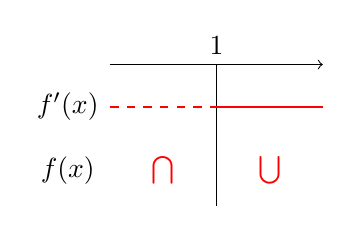
\begin{tikzpicture}[scale=0.9]
                    \draw[->](0,0)--(3,0);
                    \draw(1.5,0) node[above]{$1$}--(1.5,-2);
                    \node at (-0.6, -0.60){$f'(x)$};
                    \node at (-0.6, -1.50){$f(x)$};
                    \node[red] at (0.75,-1.50) {$\bigcap$};
                    \node[red] at (2.25,-1.50) {$\bigcup$};
                    \node[red] at (1.5, -0.60) {$\nexists$};
                    \draw[red,dashed] (0,-0.6)--(1.5,-0.6);
                    \draw[red] (1.5,-0.6)--(3,-0.6);
                \end{tikzpicture}
            \end{center}
        \item \textbf{Estremi globali: }per quanto detto precedentemente possiamo affermare che la funzione è illimitata sia inferiormente che superiormente. Non emmette perciò estremi globali.
        \item \textbf{Grafico:} ora abbiamo tutte le informazioni sufficienti per completare il grafico della funzione. Se abbiamo svolto il lavoro correttamente, ogni informazione acquisita deve essere stata confermata dalle precedenti. Si consiglia di aggiornare il disegno per ogni nuova informazione acquisita in modo da confrontarla con le precedenti. Anche per questo è stato scelto di proporre questo ordine.
        \begin{center}
            \begin{tikzpicture}[line cap=round,line join=round,>=triangle 45,x=1.0cm,y=1.0cm]
            \begin{axis}[
            x=1.0cm,y=1.0cm,
            axis lines=middle,
            ymajorgrids=true,
            xmajorgrids=true,
            xmin=-5.5,
            xmax=7.5,
            ymin=-3.5,
            ymax=6.5,
            xtick={-5.0,-4.0,...,7.0},
            ytick={-3.0,-2.0,...,6.0},]
            \clip(-5.5,-3.5) rectangle (7.5,6.5);
            \fill[line width=0.pt,color=blue,fill=blue,fill opacity=0.10000000149011612] (1.,0.) -- (1.,15.043627143200652) -- (-14.043627143200649,15.043627143200652) -- (-14.043627143200652,0.) -- cycle;
            \fill[line width=0.pt,color=blue,fill=blue,fill opacity=0.10000000149011612] (1.,0.) -- (1.,-15.043627143200652) -- (16.043627143200645,-15.043627143200654) -- (16.043627143200652,0.) -- cycle;
            \draw[line width=2.pt,color=teal,smooth,samples=100,domain=-5.5:0.9] plot(\x,{(\x)^(2)/((\x)-1)});
            \draw[line width=2.pt,color=teal,smooth,samples=100,domain=1.1:5.5] plot(\x,{(\x)^(2)/((\x)-1)});
            \draw[line width=1.pt,dash pattern=on 5pt off 5pt,color=red,smooth,samples=100,domain=-5.5:5.5] plot(\x,{(\x)+1});
            \draw [line width=1.pt,dash pattern=on 5pt off 5pt,color=red] (1.,-3.5) -- (1.,6.5);
            \draw [line width=0.pt,color=blue] (1.,0.)-- (1.,15.043627143200652);
            \draw [line width=0.pt,color=blue] (1.,15.043627143200652)-- (-14.043627143200649,15.043627143200652);
            \draw [line width=0.pt,color=blue] (-14.043627143200649,15.043627143200652)-- (-14.043627143200652,0.);
            \draw [line width=0.pt,color=blue] (-14.043627143200652,0.)-- (1.,0.);
            \begin{scriptsize}
            \draw [fill=black] (0.,0.) circle (2.5pt);
            \draw[color=black] (0.2,0.3) node {$O$};
            \draw [fill=black] (2.,4.) circle (2.5pt);
            \draw[color=black] (2.2,4.3) node {$M$};
            \end{scriptsize}
            \end{axis}
            \end{tikzpicture}
        \end{center}
        \end{enumerate}
    \end{ex}

    \begin{ex}
        [Studiare la funzione $y=x-\sqrt{x^2+4x}$, tralasciando la derivata seconda.]
        \begin{enumerate}
            \item \textbf{Classificazione:} funzione algebrica razionale fratta.
            \item \textbf{Dominio:} $x^3+4x\geq 0\ \ \Harr \ \ x(x+4)\geq 0\ \ ]-\infty;-4]\ \cup \ [0;+\infty[$
            \item \textbf{Simmetrie:} la condizione necessaria non è rispettata, per cui la funzione non è né pari né dispari.
            \item \textbf{Intersezioni con gli assi:} 
            \[\begin{cases}
                y=0\\
                y=f(x)
            \end{cases}\ \Harr \ \ x-\sqrt{x^2+4x}=0\ \ \Harr \ \ \sqrt{x^2+4x}=x\ \ \Harr\ \ \begin{cases}
                x(x+4)\geq 0\\
                x\geq 0\\
                x^2+4x=x^2
            \end{cases}\ \ \Harr\ \ \begin{cases}
                x\geq 0\\
                4x=0
            \end{cases}\]
            Per cui la funzione interseca gli assi cartesiani nell'origine $O(0,0)$.
            \item \textbf{Segno: }$f(x)>0$
            \[x-\sqrt{x^2+4x}>0\ \ \Harr\ \  \sqrt{x^2+4x}<x \ \ \Harr \ \ \begin{cases}
                x^4+4x\geq 0\\
                x>0\\
                x^2+4x<x^2
            \end{cases}\ \ \Harr \ \ \begin{cases}
                x\leq -4 \lor \geq 0\\
                x>0\\
                x<0
            \end{cases}\Harr\ \varnothing\]
            Per cui la funzione è negativa in tutto il suo dominio.
            \item \textbf{Limiti, asintoti e discontinuità:} Dobbiamo calcolare i limiti agli estremi del dominio.
            \[\lim_{x\to-\infty}\left( x-\sqrt{x^2+4x} \right)=-\infty\]
            È verificata la condizione necessaria per la presenza dell'asintoto obliquo. Procediamo con la verifica:
            \[m=\lim_{x\to -\infty}\frac{x-\sqrt{x^2-4x}}{x}=\left[ \frac{\infty}{\infty} \right]\underset{ger.}{\overset{FI}{=}}\lim_{x\to -\infty}\frac{x-\sqrt{x^2}}{x}=\lim_{x\to -\infty}\frac{x-|x|}{x}=\lim_{x\to -\infty}\frac{2x}{x}=2\]
            \[\begin{aligned}
                q&=\lim_{x\to -\infty}\left(x-\sqrt{x^2-4x}-2x\right)=\lim_{x\to -\infty}\left(-\sqrt{x^2-4x}-x\right)=\left[{-\infty+\infty} \right]\overset{FI}{=}\\
                &=\lim_{x\to-\infty}-\frac{x^2+4x-x^2}{\sqrt{x^2+4x}-x}\underset{ger.}{=}\lim_{x\to-\infty}-\frac{4x}{\sqrt{x^2}-x}= \lim_{x\to-\infty}-\frac{4x}{|x|-x}= \lim_{x\to-\infty}-\frac{4x}{-x-x}= 2
            \end{aligned}\]
            La funzione presenta quindi un asintoto obliquo sinistro alla retta $y=2x+2$.
            \[\lim_{x\to -4^-}\left( x-\sqrt{x^2+4x} \right)=-4^-\qquad \qquad f(-4)=-4\]
            la funzione è quindi continua da sinistra in $x=-4$;
            \[\lim_{x\to 0^+}\left( x-\sqrt{x^2+4x} \right)=0^-\qquad \qquad f(0)=0\]
            la funzione è quindi continua da destra in $x=0$.
            \[\begin{aligned}\lim_{x\to+\infty}\left( x-\sqrt{x^2+4x} \right)&=\left[{-\infty+\infty} \right]\overset{FI}{=}\lim_{x\to+\infty}\frac{x^2-x^2-4x}{x+\sqrt{x^2+4x}}=\left[ \frac{\infty}{\infty} \right]\underset{ger.}{\overset{FI}{=}}\lim_{x\to+\infty}\frac{-4x}{x+\sqrt{x^2}}=\\&=\lim_{x\to +\infty}\frac{-4x}{2x}=-2\end{aligned}\]
            La funzione presenta quindi un asintoto orizzontale destro alla retta $y=2$.
            \item \textbf{Derivata prima: }
            \[y'=1-\frac{1}{2\sqrt{x^2+4x}}\left( 2x+4 \right)=\frac{\sqrt{x^2+4x}-x-2}{\sqrt{x^2+4x}}\]
            Determiniamo il dominio della derivata prima $\dom f'=]-\infty;-4[\ \cup \ ]0;+\infty[$ e osserviamo che differisce dal dominio della funzione per i punti $x=0$ e $x=-4$. Essi saranno dei punti di non derivabilità da classificare. Posso applicare il criterio di derivabilità:
            \[f'_-(-4)=\lim_{x\to -4^-}\frac{\sqrt{x^2+4x}-x-2}{\sqrt{x^2+4x}}=\left[\frac{2}{0^+}\right]=+\infty\qquad \qquad f'_+(-4)\ \nexists \text{ per dominio}\]
            la funzione presenta un punto a tangente verticale in $x=-4$;
            \[f'_-(0)\ \nexists \text{ per dominio}\qquad \qquad f'_+(0)=\lim_{x\to 0}\frac{\sqrt{x^2+4x}-x-2}{\sqrt{x^2+4x}}=\left[\frac{-2}{0^+}\right]=-\infty\]
            la funzione presenta un punto a tangente verticale in $x=0$. Cerchiamo ora eventuali punti stazionari:
            \[\frac{\sqrt{x^2+4x}-x-2}{\sqrt{x^2+4x}}=0\qquad {\sqrt{x^2+4x}=x+2}\qquad \begin{cases}
                x(x+4)\geq 0\\
                x\geq -2\\
                x^2-4x=x^2-4x+4
            \end{cases}\ \  \begin{cases}
                x(x+4)\geq 0\\
                x\geq -2\\
                0=4
            \end{cases}\]
            La funzione non ha quindi punti stazionari. Studiamo ora il segno della derivata:
            \begin{center}
                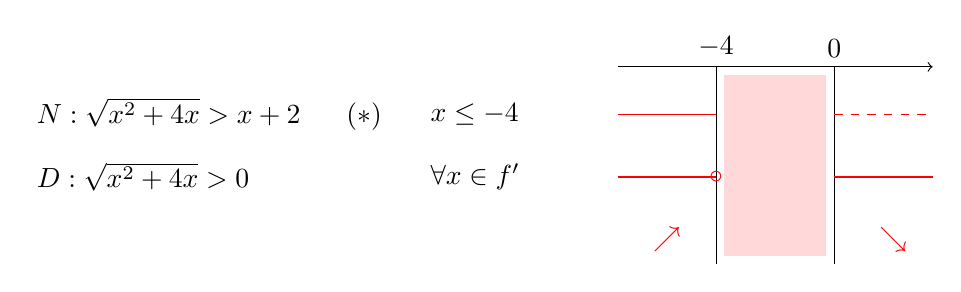
\begin{tikzpicture}
                    \fill [red!15] (8.85,0.9)--(8.85,-1.4)--(10.15,-1.4)--(10.15,0.9)--cycle;
                    \node at (0,0.4) [anchor=west]{$N: \sqrt{x^2+4x}>x+2\quad~~ (*)$};
                    \node at (0,-0.4)[anchor=west]{$D: \sqrt{x^2+4x}>0$};
                    \node at (5,0.4)[anchor=west]{$x\leq -4$};
                    \node at (5,-0.4)[anchor=west]{$\forall x \in \dom f'$};
                    \draw[->] (7.5,1)--(11.5,1);
                    \draw (8.75,1)node [above]{$-4$}--(8.75,-1.5);
                    \draw (10.25,1) node [above]{$0$}--(10.25,-1.5);
                    %%riga 1
                    \draw [color=red] (7.5, 0.4)--(8.75,0.4);
                    \node [color=red] at (8.75,0.4){$\nexists$};
                    \draw [color=red, dashed] (10.25, 0.4)--(11.5,0.4);
                    \node [color=red] at (10.25,0.4){$\nexists$};
                    %% riga 2
                    \draw[color=red] (7.5, -0.4)--(8.75,-0.4) node {$\circ$};
                    \draw [color=red] (10.25, -0.4)--(11.5,-0.4);
                    
                    \node [color=red]at (8.125,-1.2){$\nearrow$};
                    \node [color=red]at (11,-1.2){$\searrow$};
                \end{tikzpicture}
            \end{center}
            \[(*)\qquad \begin{cases}
                x^2+4x\geq 0\\x+2\geq 0\\ x^2+4x>(x+2)^2
            \end{cases}\quad \cup \qquad \begin{cases}
                x^2+4x\geq 0\\x+2<0\\\forall x \in \R
            \end{cases}\]
            \[\varnothing\quad \cup \quad x\leq -4\]
            \addtocounter{enumi}{1} % skip derivata seconda
            \item \textbf{Estremi globali: } La funzione ha punti di massimo globali in $x=-4$ e $x=0$; è illimitata inferiormente.
            \item \textbf{Disegno: }
            \begin{center}
                \begin{tikzpicture}[line cap=round,line join=round,>=triangle 45,x=1.0cm,y=1.0cm]
                \begin{axis}[
                x=1.0cm,y=1.0cm,
                axis lines=middle,
                ymajorgrids=true,
                xmajorgrids=true,
                xmin=-6.5,
                xmax=5.5,
                ymin=-7.5,
                ymax=1.5,
                xtick={-6.0,-5.0,...,5.0},
                ytick={-7.0,-6.0,...,1.0},]
                \clip(-7.5,-7.5) rectangle (7.5,1.5);
                \fill[line width=0.pt,color=blue,fill=blue,fill opacity=0.10000000149011612](0,0)--(6,0)--(6,2)--(0,2)--cycle;
                \fill[line width=0.pt,color=blue,fill=blue,fill opacity=0.10000000149011612](-4,0)--(-6.5,0)--(-6.5,2)--(-4,2)--cycle;
                \fill[line width=1.5pt,dash pattern=on 5pt off 2pt,color=red,fill=red,fill opacity=0.10000000149011612] (-4.,8.) -- (0.,8.) -- (0.,-18.) -- (-4.,-18.) -- cycle;
                \draw[line width=2.pt,color=teal,smooth,samples=100,domain=-5.5:-4.000000069999991] plot(\x,{(\x)-sqrt((\x)^(2.0)+4*(\x))});
                \draw[line width=2.pt,color=teal,smooth,samples=100,domain=9.248943717311174E-6:5.5] plot(\x,{(\x)-sqrt((\x)^(2.0)+4*(\x))});
                \draw[line width=1.5pt,dash pattern=on 5pt off 5pt,color=red,smooth,samples=100,domain=-5.5:-4] plot(\x,{2*(\x)+2});
                \draw [line width=1.5pt,dash pattern=on 5pt off 5pt,color=red,domain=0:5.5] plot(\x,{(-2.-0.*\x)/1.});
                \draw [line width=1.5pt,dash pattern=on 5pt off 5pt,color=red] (-4.,8.)-- (0.,8.);
                \draw [line width=1.5pt,dash pattern=on 5pt off 5pt,color=red] (0.,8.)-- (0.,-18.);
                \draw [line width=1.5pt,dash pattern=on 5pt off 5pt,color=red] (0.,-18.)-- (-4.,-18.);
                \draw [line width=1.5pt,dash pattern=on 5pt off 5pt,color=red] (-4.,-18.)-- (-4.,8.);
                \begin{scriptsize}
                \draw [fill=blue] (0.,0.) circle (2.5pt);
                \draw[color=blue] (0.11658212836203329,0.29260536954385497) node {$O$};
                \end{scriptsize}
                \end{axis}
                \end{tikzpicture}
            \end{center}
        \end{enumerate}
    \end{ex}

\section{Esercizi}
    \begin{exc}\label{exc: sfx 1}
        Studiare la funzione $\displaystyle g(x)=e^{\left|\frac{x+1}{x-1}\right|}$.\qquad {\hyperref[sol: sfx 1]{\footnotesize Soluzione a pag. \pageref*{sol: sfx 1}}}
    \end{exc}

    \begin{exc}\label{exc: sfx 2}
        Sia $g(x)=|x-1|e^{-\alpha x} ~~(\alpha>0)$. Fornire un grafico qualitativo di $g$.\qquad {\hyperref[sol: sfx 2]{\footnotesize Soluzione a pag. \pageref*{sol: sfx 2}}}
    \end{exc}